% vim: set spell spelllang=en tw=100 et sw=4 sts=4 :

\documentclass[a2paper]{tikzposter}

\usepackage{microtype}
\usepackage{tikz}
\usepackage{amssymb}
\usepackage{amsmath}
\usepackage{pifont}

\usepackage{lmodern}
\renewcommand*\familydefault{\sfdefault}
\usepackage[T1]{fontenc}

\usetikzlibrary{positioning, backgrounds, scopes, calc, fit, graphs, graphs.standard, shapes.geometric,
shapes.multipart, arrows, arrows.meta}

\title{Auditable Algorithms}
\author{Arthur Gontier, Ciaran McCreesh, and
Matthew McIlree}
\institute{University of Glasgow, Glasgow, Scotland}

\settitle{
    \begin{tikzpicture}
        \node (T) [inner xsep=0pt, inner ysep=-20pt] {\begin{minipage}{\linewidth}
                \color{titlefgcolor}
                {\bfseries \huge \@title \par}
                \vspace*{0.6em}
                {\large {\bfseries \@author} \\[0.1em] \@institute}
                \vspace*{0.6em}

                {\small With numerous co-conspirators, including Bart
                Bogaerts (VU Brussels), Emir Demirovi\'c and \\ Konstatntin Sidorov (TU Delft), Stephan
                Gocht, Jakob Nordstr{\"o}m and Andy Oertel (Lund \\ University and University of
                Copengagen), Magnus O. Myreen (Chalmers University), and \\
                Yong Kiam Tan (I$^2$R, A$\star$STAR)}
        \end{minipage}};

        \coordinate (logopos) at (T.east);

        \node at (logopos) [anchor=center, inner sep=0pt, xshift=0cm, yshift=2.3cm,
        xshift=-5.5cm] {
            \includegraphics[keepaspectratio=true,height=3.0cm]{../../images/UoG_keyline.pdf}
        };

        \node at (logopos) [anchor=center, inner sep=0pt, xshift=0cm, yshift=-2.3cm,
        xshift=-5.5cm] {
            \includegraphics[keepaspectratio=true,height=3.0cm]{../../images/RAEngWhite.pdf}
        };
    \end{tikzpicture}
}

% University of Glasgow standard colours
\definecolor{uofguniversityblue}{rgb}{0, 0.219608, 0.396078}

\definecolor{uofgheather}{rgb}{0.356863, 0.32549, 0.490196}
\definecolor{uofgaquamarine}{rgb}{0.603922, 0.72549, 0.678431}
\definecolor{uofgslate}{rgb}{0.309804, 0.34902, 0.380392}
\definecolor{uofgrose}{rgb}{0.823529, 0.470588, 0.709804}
\definecolor{uofgmocha}{rgb}{0.709804, 0.564706, 0.47451}

\definecolor{uofglawn}{rgb}{0.517647, 0.741176, 0}
\definecolor{uofgleaf}{rgb}{0, 0.517647, 0.239216}
\definecolor{uofgcobalt}{rgb}{0, 0.615686, 0.92549}
\definecolor{uofgturquoise}{rgb}{0, 0.709804, 0.819608}
\definecolor{uofgsunshine}{rgb}{1.0, 0.862745, 0.211765}
\definecolor{uofgpumpkin}{rgb}{1.0, 0.72549, 0.282353}
\definecolor{uofgthistle}{rgb}{0.584314, 0.070588, 0.447059}
\definecolor{uofgpillarbox}{rgb}{0.701961, 0.047059, 0}
\definecolor{uofglavendar}{rgb}{0.356863, 0.301961, 0.580392}

\definecolor{uofgsandstone}{rgb}{0.321569, 0.278431, 0.231373}
\definecolor{uofgforest}{rgb}{0, 0.317647, 0.2}
\definecolor{uofgburgundy}{rgb}{0.490196, 0.133333, 0.223529}
\definecolor{uofgrust}{rgb}{0.603922, 0.227451, 0.023529}

\definecolorstyle{UofG}{
}{
    % Background Colors
    \colorlet{backgroundcolor}{uofgsandstone!80!white}
    \colorlet{framecolor}{black}
    % Title Colors
    \colorlet{titlefgcolor}{white}
    \colorlet{titlebgcolor}{uofguniversityblue}
    % Block Colors
    \colorlet{blocktitlebgcolor}{white}
    \colorlet{blocktitlefgcolor}{uofguniversityblue}
    \colorlet{blockbodybgcolor}{white}
    \colorlet{blockbodyfgcolor}{black}
    % Innerblock Colors
    \colorlet{innerblocktitlebgcolor}{uofguniversityblue}
    \colorlet{innerblocktitlefgcolor}{black}
    \colorlet{innerblockbodybgcolor}{uofgsandstone}
    \colorlet{innerblockbodyfgcolor}{black}
    % Note colors
    \colorlet{notefgcolor}{black}
    \colorlet{notebgcolor}{uofgrust}
    \colorlet{noteframecolor}{red}
}

\usetheme{Autumn}
\usecolorstyle{UofG}

\tikzposterlatexaffectionproofoff

\useblockstyle[bodyverticalshift=-1cm, roundedcorners=1]{Default}

\renewcommand{\Huge}{\fontsize{77.2}{96}\selectfont}

% Styles for drawings

\tikzset{edge/.style={line width=3pt, color=uofgsandstone}}
\tikzset{ledge/.style={line width=3pt, color=uofgsandstone!40!white}}

\setlength\intextsep{0pt}

\begin{document}
\maketitle

{
    \colorlet{blockbodybgcolor}{uofgcobalt}
    \colorlet{blocktitlebgcolor}{uofgcobalt}
    \block[bodyverticalshift=0cm, bodyinnersep=3mm]{}{
        \centering\begin{minipage}{0.90\textwidth}
            \textbf{Why should you believe an algorithm is giving you the right answer?}
            Increasingly complex ``intelligent'' algorithms are being deployed in ways that
            directly affect your life and livelihood, and often no-one knows whether these algorithms are
            designed and implemented correctly. We can fix this by
            \textbf{trusting solutions, not solvers}: by making solving algorithms show their
            work in a verifiable way, we can \textbf{independently audit solutions} for correctness
            and optimality. This does not mean an algorithm is free from bugs or maliciousness, but
            it does mean that if it ever gives a wrong answer, it can always be detected.
        \end{minipage}
    }
}

\block{From Problem Description to a Trusted Solution}{
    \centering
    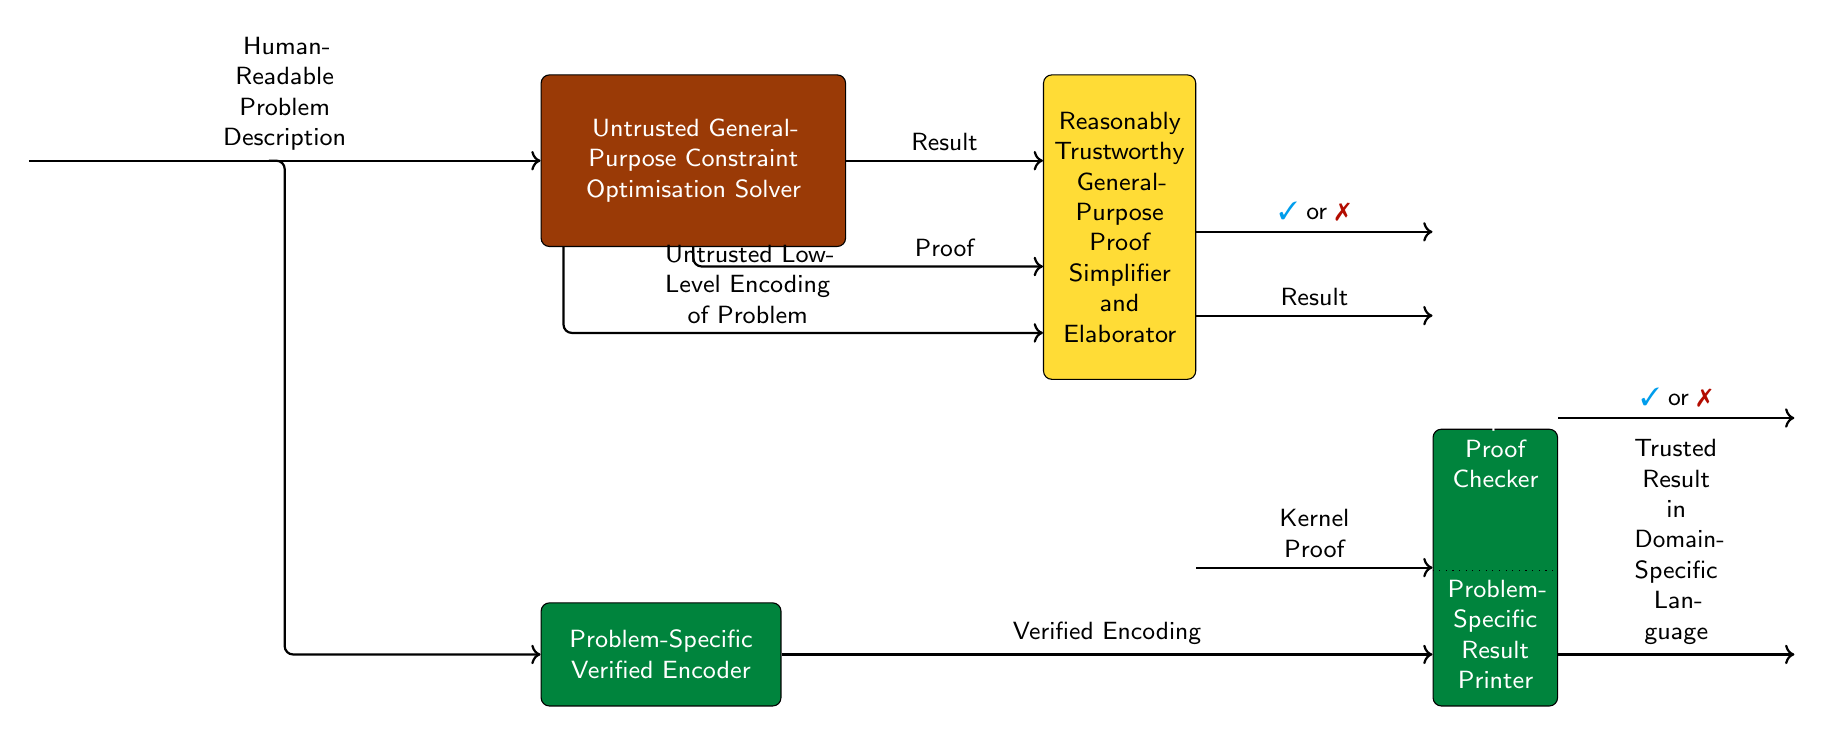
\begin{tikzpicture}[font=\small]
        \node (solver) [text centered, text width=10em, inner xsep=0.5em, inner ysep=1.6em, draw, rounded
        corners=3pt, fill=uofgrust, text=white] { Untrusted General-Purpose Constraint Optimisation Solver};

        \node (elaborator) [ right=2.5cm of solver.north east, anchor=north west, inner
        xsep=0.25em, draw, rounded corners=3pt, minimum height=11em, text width=5em, text centered,
        fill=uofgsunshine]
        { Reasonably Trustworthy General-Purpose Proof Simplifier and Elaborator };

        \node (verifiedchecker) [ right=3cm of elaborator.north east, anchor=north west, inner
            xsep=0.25em, draw, rounded corners=3pt, minimum height=10em, text width=4em, text
            centered, yshift=-4.5cm, fill=uofgleaf, text=white] { \phantom{Verified General-Purpose Proof Checker} };
        \node (gpverifiedchecker) [yshift=1.9cm, text width=4em, text centered, text=white] at (verifiedchecker)
            {Verified General-Purpose Proof Checker};
        \node (resultoutput) [anchor=south, yshift=0.3em, text width=4em, text centered, text=white] at (verifiedchecker.south)
            {Problem-Specific Result Printer};

        \node (verifiedencoder) [ draw, rounded corners=3pt, text centered, anchor=south west,
        text width=8em, inner ysep=1em, fill=uofgleaf, text=white] at (solver.west|-verifiedchecker.south) {
            Problem-Specific Verified Encoder };

        \draw [->, thick] (solver.east) -- (solver.east -| elaborator.west)
            coordinate [midway] (solutionmid) node [above, midway] { Result };

        \coordinate (elaboratorproofin) at ($(elaborator.west)+(0,-0.5)$);

        \draw [->, thick, rounded corners=3pt] (solver.south) -- (solver.south |- elaboratorproofin)
            -- (elaboratorproofin) coordinate [midway] (proofmid);

        \coordinate (prooflabel) at (proofmid-|solutionmid);
        \node [above=0cm of prooflabel] { Proof };

        \coordinate [right=3cm of verifiedchecker.east] (verified);
        \draw [->, thick] (verifiedchecker.east|-gpverifiedchecker.east) --
        (verified|-gpverifiedchecker.east)
            node [above, midway] { \textcolor{uofgcobalt}{\ding{51}} or \textcolor{uofgpillarbox}{\ding{55}} };

        \coordinate (verifiedcheckertopleft) at ($(verifiedchecker.west)+($(0cm,3.2cm)$)$);
        \draw [->, thick] (elaborator.east |- verifiedcheckertopleft) -- (verifiedcheckertopleft) node [above, midway, text width=4em, text centered] { Result };
        \draw [->, thick] (elaborator.east |- verifiedchecker.west) -- (verifiedchecker.west) node [above, midway, text width=3em, text centered] { Kernel Proof };

        \coordinate (elaboratortopright) at ($(elaborator.north east)+(0.0,-2.0)$);
        \draw [->, thick] (elaboratortopright) -- (elaboratortopright-|verifiedchecker.west)
            node [above, midway] { \textcolor{uofgcobalt}{\ding{51}} or \textcolor{uofgpillarbox}{\ding{55}} };

        \coordinate [left=6.5cm of solver.west] (input);
        \draw [->, thick] (input) -- (solver.west) coordinate [midway] (inputmid) node [above,
        midway, text width=6em, text centered] { Human-Readable Problem Description };

        \coordinate (checkerbotleft) at
        ($(elaborator.west)+($(elaborator.west)-(solver.east-|elaborator.west)+(0,-0.5)$)$);

        \coordinate (solverstart) at ($(solver.south)!0.85!(solver.south west)$);
        \coordinate (solverstart2) at ($(solver.south)!0.75!(solver.south west)$);
        \draw [->, thick, rounded corners=3pt] (solverstart) -- (solverstart |- checkerbotleft) -- (checkerbotleft)
        coordinate [midway] (altinputmid);

        \coordinate (encinputlabel) at (altinputmid-|solutionmid);
        \node [above=0cm of encinputlabel, xshift=-2.5cm, text width=8em, text centered] { Untrusted
        Low-Level Encoding of Problem };

        \draw [->, thick, rounded corners=3pt] ($(inputmid)+(-0.2,0)$) -- (inputmid) -- (inputmid |-
        verifiedencoder.west) -- (verifiedencoder.west);

        \draw [->, thick] (verifiedencoder.east) -- (verifiedchecker.west|-verifiedencoder.east)
        node [above, midway] { Verified Encoding };

        \draw [->, thick] (verifiedchecker.east|-verifiedencoder.west) -- (verified|-verifiedencoder.west)
            node (trustedresult) [above, midway, text centered, text width=3em] { Trusted Result in
            Domain-Specific Language };

        \draw [dotted]
        (verifiedchecker.west|-resultoutput.north)--(verifiedchecker.east|-resultoutput.north);

    \end{tikzpicture}
}

\begin{columns}
\column{0.55}

\block{Why is this Hard?}{
    Proofs need to be expressive, to efficiently capture all the reasoning carried out by intelligent
    combinatorial optimisation algorithms. But proof steps must also be simple, so that we can trust
    the proof system and checker.
}

\column{0.45}

\block{Further Reading}{
    \scriptsize
SG, CM, MOM, JN, AO, YKT: End-to-End Verification for Subgraph Solving. AAAI 2024.

BB, SG, CM, JN:
Certified Dominance and Symmetry Breaking for Combinatorial Optimisation. J. Artif. Intell. Res. 77. (2023)

MJM, CM:
Proof Logging for Smart Extensional Constraints. CP 2023.

SG: Certifying Correctness for Combinatorial Algorithms: by Using Pseudo-Boolean Reasoning. Lund
University, Sweden, 2022. PhD Thesis.

SG, CM, JN:
An Auditable Constraint Programming Solver. CP 2022.
}
\end{columns}

{
    \colorlet{blockbodybgcolor}{uofgsandstone!80!white}
    \colorlet{blocktitlebgcolor}{uofgsandstone!80!white}
    \block[bodyverticalshift=-1.5cm]{}{\small
On two occasions I have been asked, -- ``Pray, Mr. Babbage, if you put into the machine wrong
figures, will the right answers come out?'' I am not able rightly to apprehend the kind of confusion
of ideas that could provoke such a question. \\
        This work is supported by a Royal Academy of Engineering Research Fellowship, and by the Engineering and Physical Sciences Research Council [grant number
        EP/X030032/1]. \hfill \texttt{\textcolor{white}{ciaran.mccreesh@glasgow.ac.uk}} \\
    }
}

\end{document}

